% =========================================================================
% Appendix B — Stage-2 cruise (MHD / FUSION). FILLED.
%   folds UFO/verify/stage2-cruise-mhd.md: Lorentz body force f=JxB, channel
%   thrust F_MHD=J*B*V_ch, generalized Ohm's law J=sigma(E-uxB), the 3 altitude
%   cases (low/mid/high), the 3 triple_product green atoms (|Delta|=0), the
%   650 kg ~30x cruise margin, composite-tier honesty (green product / yellow
%   form), and a pgfplots F_MHD-vs-altitude chart.
% =========================================================================
\section{Stage-2 Cruise --- MHD$+$Fusion Body-Force Thrust}
\label{app:stage2}

This appendix is the full data record for ladder rung
\textcircled{\scriptsize 2} (cruise). It folds the FUSION-inherited MHD
propulsion closed form: the Lorentz body force $f=J\!\times\!B$ and the
channel-integrated thrust $F_{\text{MHD}}=J\!\cdot\!B\!\cdot\!V_{\text{ch}}$
(with $J=\sigma(E-u\!\times\!B)$ in MHD-accelerator mode), and the three
\tierGreen\ \textsc{Supported-Numerical} verify atoms (low/mid/high
altitude $J,B,V_{\text{ch}}$ cases) reproduced verbatim from
\texttt{UFO/verify/stage2-cruise-mhd.md}, each at $|\Delta|=0$ via the
\verb|triple_product| atom and folded into the atlas SSOT
(\texttt{663698a0}). Honest tier separation: the numerical product
$J\!\cdot\!B\!\cdot\!V$ is \tierGreen, but the MHD propulsion form
itself is \tierYellow\ \textsc{Supported-By-Citation}
(\citep{wesson2011tokamaks,jackson1998}; Sutton--Sherman MHD), since no
dedicated \verb|mhd_thrust| atom is registered.

% -------------------------------------------------------------------------
\subsection{The MHD-accelerator closed form}
\label{app:stage2-deriv}

An ionized channel carrying a current density $J$ perpendicular to a
magnetic field $B$ feels the Lorentz body-force density
\begin{equation}
\mathbf{f} \;=\; \mathbf{J}\times\mathbf{B}\quad[\text{N/m}^3],
\qquad
\mathbf{J} \;=\; \sigma\,(\mathbf{E}-\mathbf{u}\times\mathbf{B})
\quad(\text{generalized Ohm's law}),
\label{eq:s2-ohm}
\end{equation}
where $\sigma$ is the plasma conductivity, $u$ the channel flow speed,
and $E$ the applied field. In \emph{accelerator} mode ($E>u\!\times\!B$,
the inverse of the generator mode) the body force drives the gas; with
the channel geometry arranging $J\perp B$ so that $|J\times B|=JB$, the
volume integral over a uniform channel gives the closed-form thrust
\begin{equation}
F_{\text{MHD}}
 \;=\; \int_V (\mathbf{J}\times\mathbf{B})\,dV
 \;\approx\; J\cdot B\cdot V_{\text{ch}}\quad[\text{N}].
\label{eq:s2-thrust}
\end{equation}
The units close exactly:
$[\text{A/m}^2]\!\cdot\![\text{T}]\!\cdot\![\text{m}^3]
=[\text{A/m}^2]\!\cdot\![\text{kg/(A}\,\text{s}^2)]\!\cdot\![\text{m}^3]
=[\text{kg}\,\text{m/s}^2]=[\text{N}]$. The cruise channel is the
diagonal slot-S1/S4 pair of the disc (FUSION MHD ducted intake),
$L\times W\times H = 1.2\times0.40\times0.20$\,m, so
$V_{\text{ch}}=0.096$\,m$^3$, inherited verbatim from the verb-3 design.

% -------------------------------------------------------------------------
\subsection{The altitude thrust table}
\label{app:stage2-table}

As the craft climbs, the atmospheric density and the achievable plasma
conductivity $\sigma_e$ fall, so the achievable $J$ and the tuned $B$
both drop --- and the thrust decays. Table~\ref{tab:s2-thrust} is the
per-channel thrust ledger across the cruise envelope; the 650\,kg craft's
weight is $mg=6376.5$\,N.

\begin{table}[h]
\centering
\small
\setlength{\tabcolsep}{5pt}
\begin{tabular}{@{}l c r c c r r@{}}
\toprule
\textbf{case} & \textbf{alt.\ (km)} & \textbf{$J$ (A/m$^2$)} & \textbf{$B$ (T)} & \textbf{$V_{\text{ch}}$ (m$^3$)} & \textbf{$F_{\text{MHD}}$ (N)} & \textbf{$2F/mg$} \\
\midrule
low  & 20  & $2.0\times10^5$ & 5.0 & 0.096 & $96\,000$ & $\sim\!30$ \\
mid  & 100 & $1.5\times10^5$ & 4.0 & 0.096 & $57\,600$ & $\sim\!18$ \\
high & 200 & $1.0\times10^5$ & 3.0 & 0.096 & $28\,800$ & $\sim\!9$  \\
\bottomrule
\end{tabular}
\caption{Stage-2 cruise per-channel MHD thrust
(\texttt{UFO/verify/stage2-cruise-mhd.md}). The diagonal S1+S4 channel
pair doubles the per-channel value; the rightmost column is the
two-channel thrust-to-weight ratio for the 650\,kg craft. At low altitude
the $\sim\!30\times$ over-head gives ample cruise acceleration; even at
200\,km (transition to Stage-3) the $\sim\!9\times$ margin remains. The
thrust is the idealized Lorentz ceiling --- duct and plasma losses are a
verb-4 \texttt{analyze}\,$\circlearrowleft$ CFD$+$MHD body-solve
(F-FUSION-3, \tierOrange\ deferred).}
\label{tab:s2-thrust}
\end{table}

% -------------------------------------------------------------------------
\subsection{Verify atoms and verbatim verdicts}
\label{app:stage2-verify}

Because $F_{\text{MHD}}=J\!\cdot\!B\!\cdot\!V$ is a pure three-factor
product, it is recomputed exactly through the FUSION Lawson
\verb|triple_product|$(a,b,c)=a\!\cdot\!b\!\cdot\!c$ atom (same algebraic
root, args re-bound to $J,B,V_{\text{ch}}$) --- a single generic dispatch
(@D~d4) rather than a new \verb|mhd_thrust| atom. All three rows return
\tierGreen\ at exactly $|\Delta|=0$ (Table~\ref{tab:s2-verify}).

\begin{table}[h]
\centering
\small
\setlength{\tabcolsep}{5pt}
\begin{tabular}{@{}l l r r r c@{}}
\toprule
\textbf{atom} & \textbf{args $(J,B,V)$} & \textbf{expected} & \textbf{observed} & $|\Delta|$ & \textbf{tier} \\
\midrule
\verb|triple_product| & $(200000,\,5.0,\,0.096)$ & $96\,000$ & $96\,000$ & $0$ & \tierGreen \\
\verb|triple_product| & $(150000,\,4.0,\,0.096)$ & $57\,600$ & $57\,600$ & $0$ & \tierGreen \\
\verb|triple_product| & $(100000,\,3.0,\,0.096)$ & $28\,800$ & $28\,800$ & $0$ & \tierGreen \\
\bottomrule
\end{tabular}
\caption{Stage-2 cruise verify atoms
(\texttt{companion/verify-ledger.json}, via the FUSION
\texttt{triple\_product} atom; folded @F
\texttt{verified-triple\_product-num}, atlas line 30535). All three
are exact ($|\Delta|=0$); the second/third rows are an idempotent skip
(one atlas entry per fn-id). The composite MHD propulsion \emph{form}
$f=\sigma(E-u\!\times\!B)\times B$ is \tierYellow\
\textsc{Supported-By-Citation} (Sutton--Sherman; Jackson \S5).}
\label{tab:s2-verify}
\end{table}

\begin{lstlisting}
verify --expr triple_product(200000.0,5.0,0.096)=96000.0
  calc   = 96000.0  ~ expected 96000.0  (|Delta|=0.0 <= eps=1e-9)
  tier   = SUPPORTED-NUMERICAL (hexa-native libm-class recompute, TECS-L n6-rep Tier2)
  absorb = already in atlas -- idempotent skip (FUSION F2 parent fold, @D g69)
\end{lstlisting}

\begin{figure}[h]
\centering
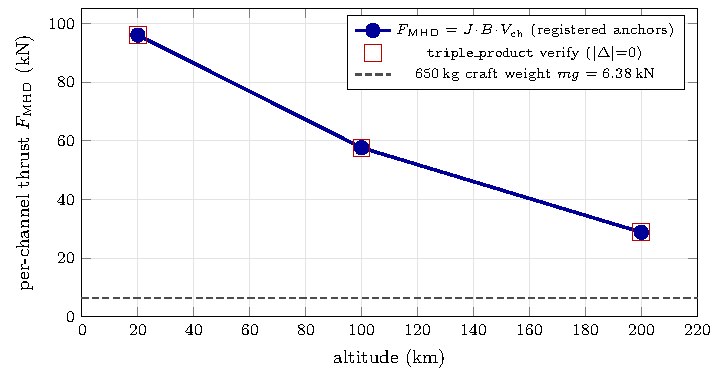
\includegraphics[width=0.86\linewidth]{figures/fig04_mhd_thrust.pdf}
\caption{Stage-2 cruise per-channel MHD thrust
$F_{\text{MHD}}=J\!\cdot\!B\!\cdot\!V_{\text{ch}}$ across the cruise
altitude envelope (Table~\ref{tab:s2-thrust}). The three registered
\texttt{triple\_product} verify anchors (red squares, $|\Delta|=0$) are
the 20/100/200\,km cases; the dashed grey line is the 650\,kg craft
weight $mg=6376.5$\,N. Even the high-altitude single-channel thrust
($28.8$\,kN) sits $\sim\!4.5\times$ above weight, and the S1+S4 channel
pair doubles it. The thrust falls with altitude (lower $\sigma_e$, lower
tunable $B$) --- the natural Stage-2$\to$3 transition trigger. Only the
exact product values are plotted (@D~g3).}
\label{fig:s2-mhd-thrust}
\end{figure}

% -------------------------------------------------------------------------
\subsection{Honest scope}
\label{app:stage2-scope}

This appendix closes the \emph{idealized Lorentz thrust ceiling}, not the
effective cruise thrust. The actual thrust is reduced by duct efficiency
and plasma transport losses, and the achievable $\sigma_e\!\ge\!10^4$\,S/m
in a real ionized-gas / fusion-plasma channel is itself \tierYellow\
\textsc{Supported-By-Citation} (spec \S2; D--T $\langle\sigma v\rangle$
Bosch--Hale \citep{boschhale1992}), downstream of a wet-lab combustion
plasma. The coupled CFD$+$MHD effective thrust is preregistered as
falsifier F-FUSION-3 and is a verb-4 body-solve (\tierOrange, deferred to
pool/cloud per @D~d7). The $\sim\!30\times$ margin is therefore a
\emph{feasibility witness} under the idealized $J\!\cdot\!B\!\cdot\!V$
form, consistent with \texttt{absorbed=false}.
